\documentclass[10pt]{amsart}
\usepackage{amsmath}
\usepackage{csquotes}
\usepackage{enumitem}
\usepackage{multicol}
\usepackage{tikz}
\usepackage{pgfplots}
\usepackage{caption}
\usepackage[margin=1in]{geometry}

\newenvironment{Figure}
{\par\medskip\noindent\minipage{\linewidth}}
{\endminipage\par\medskip}

\title{Introduction to Neural Networks}
\author{Arden Rasmussen}
\date{\today}

\begin{document}
\maketitle

\begin{abstract}
  Machine Learning is a rapidly expanding subject of research. At the center of
  this research are neural networks. Neural networks provide researchers with
  tools and methods for the construction of artificial intelligence. These
  AIs can be trained to ground breaking levels of thinking, frequently out
  reasoning leading humans in the subject. This paper provides a short
  introduction to the concept of neural networks, with emphasis on the
  mathematics of the neural networks.
\end{abstract}

\begin{multicols}{2}
  \section{Introduction}%
  \label{sec:introduction}

  A neural network is a computational model, that can be used for advanced
  decision making. The original influence for neural networks, comes from
  biology. This paper will attempt to provide an introductory comprehension of
  neural networks as a whole. This includes the three primary types of network,
  their structures, how they are trained, and how they may be implemented.

  The three primary types of neural network that we will discuss are
  \textit{Feed Forward}, \textit{Convolutional}, and \textit{Recurrent}. These
  three types of networks are frequently used in modern research. Most networks
  can be considered as some combination of these types of networks. Thus having
  an understanding of these three core networks types will greatly improve ones
  understanding of the current research of neural networks.

  \section{Structure}%
  \label{sec:structure}

  The first thing to understand with respect to neural networks is what all the
  terminology means. To do this we explain explicit what the building blocks
  of a neural network are. We explain how these blocks are assembled in the
  later sections. Generally each neural network is constructed from
  \textit{layers},  and each layer is constructed from \textit{neurons} and
  \textit{activation functions}. This structure is fairly universal among
  neural networks. The cases when a network differs from this generalized
  structure is outside of the scope of this introduction, and requires
  independent research.

  \subsection{Neuron}%
  \label{sub:neuron}

  The most basic component of a neural network is the \textit{neuron}. A single
  neuron takes input from many sources and produces a single output value. A
  single neuron takes inputs from other neurons or from external sources. For
  each input value the neuron assigns a weight associated with how important
  that value is relative to the other inputs. Then the neuron applies a
  function $f$, to the weighted sum of the input values.

  \begin{Figure}
    \begin{center}
      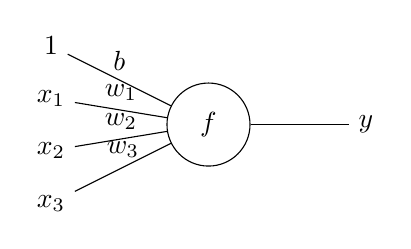
\begin{tikzpicture}[scale=1, transform shape]
  \node (i0) at (-2.0,-1.0) {$x_3$};
  \node (i1) at (-2.0,-0.33) {$x_2$};
  \node (i2) at (-2.0,0.33) {$x_1$};
  \node (i3) at (-2.0,1.0) {$1$};

  \node[circle,draw=black,fill=white,minimum size=3.0em] (n) at (0.0,0.0) {$f$};

  \node (o) at (2.0, 0.0) {$y$};

  \draw (i0) -- node[above] {$w_3$} (n);
  \draw (i1) -- node[above] {$w_2$} (n);
  \draw (i2) -- node[above] {$w_1$} (n);
  \draw (i3) -- node[above] {$b$} (n);

  \draw (n) -- (o);
\end{tikzpicture}

    \end{center}
    \captionof{figure}{A single neuron acting on inputs with provided weights
    $w_i$.}
    \label{fig:nn_single}
  \end{Figure}

  In figure \ref{fig:nn_single}, we see that the neuron takes in four inputs,
  $x_1,\ldots,x_3,1$. Then for each input there is an associated "importance"
  to that input with respect to the other inputs $w_1,\ldots,w_3,b$. This value
  is the weight of that input. The neuron takes the inputs and the weights of
  the inputs and applies the function $f$ on the weighted sum of the inputs
  \begin{align*}
    f(w_1x_1+w_2x_2+w_3x_3+b).
  \end{align*}
  We can then generalize this formula for any number of input neurons to be
  \begin{align}\label{eq:nn_neuron}
    f\left(\sum_{i=1}^Nw_ix_i+b\right).
  \end{align}
  The output of this neuron is either passed along to other neurons as inputs,
  or is the output of our network, and is given to the user.

  The function $f$ that the neuron applies to the weighted sum is called the
  \textit{activation function}. The activation function is a non-linear
  function used to introduce non-linearity into the neural network. Without the
  non-linearity then the network would be just a bunch of linear operations,
  which could be represented as a single matrix, by the introduction of the
  non-linearity we enforce that there must be many steps. This will increase
  the ability of the network to do more complex operations in the future. We
  will go into further detail on activation functions in a different section.

  There are three main \textit{types} of neurons that we will consider.
  \begin{description}
    \item[Input Neurons] Input neurons take information from external inputs,
      such as image data, and then passes that data on to the other neurons in
      the network. The input neurons do no computation, they just pass on their
      information to later neurons.
    \item[Hidden Neurons] Hidden neurons have no connection directly to input
      or output data. They only have what is provided to them from their
      previous layer, and preform the computation that was explained in section
      \ref{sub:neuron}. Then the output value is passed on, either to more
      hidden neurons or to the output neurons.
    \item[Output Neurons] The output neurons are responsible to taking the
      values passed to them by the previous layer of neurons and processing the
      values into an understandable interpretation, such as a probability. They
      then return that data to the user.
  \end{description}
  We will uses these three types of neurons to construct the neural network.

  \subsection{Activation Function}%
  \label{sub:activation_function}

  Activation functions are a method to cause some non-linearity. This
  importance comes into play when we have multiple neurons connecting into one
  another. Since each neuron individually is linear, then this connection of
  neurons will also be linear. That would mean that it could all be modeled as a
  single neuron. This is the reason as to why we need to impose the activation
  functions, to cause non-linearity in between the different neurons, so that
  the function as a whole is not linear. This means that each neuron can be
  trained to be important in the network.

  There are a number of common functions that are used for the activation
  functions. \textit{Sigmoid}, \textit{tanh}, \textit{ReLU}, and other
  variations on \textit{ReLU}. We will describe each of these possible
  activation functions in more detail below. Through usage, it has been found
  that a good default is to use \textit{ReLU}.

  \begin{description}
    \item[Sigmoid] The sigmoid activation function is defined as
      \begin{align*}
        f(x)=\sigma(x)=\frac{1}{1+e^{-x}}.
      \end{align*}
      \begin{Figure}
      \begin{center}
      \begin{tikzpicture}[scale=0.6]
        \begin{axis}[axis lines=center]
          \addplot[]{1/(1+e^(-x))};
        \end{axis}
      \end{tikzpicture}
      \end{center}
      \captionof{figure}{$\frac{1}{1+e^{-x}}$}
      \label{fig:sigmoid}
      \end{Figure}
      The sigmoid function takes any value input to it and squashes it into the
      range of $(0,1)$. However, there are some issues that arise with the
      sigmoid activation function. If the input is small or large, then the
      output becomes saturated, and the gradient of the function at those
      points is zero. This becomes an issue later when using back propagation.
      The other issue is that the output is not centered at zero, this will
      again cause issues later with back propagation.

    \item[tanh] The tanh activation function is similar to the sigmoid
      function, but is constructed to be zero centered. It is defined as
      \begin{align*}
        f(x)=\tanh(x)=\frac{e^x-e^{-x}}{e^x+e^{-x}}.
      \end{align*}
      \begin{Figure}
      \begin{center}
      \begin{tikzpicture}[scale=0.6]
        \begin{axis}[axis lines=center]
          \addplot[]{(e^x-e^(-x))/(e^x+e^(-x))};
        \end{axis}
      \end{tikzpicture}
      \end{center}
      \captionof{figure}{$\frac{e^x-e^{-x}}{e^x+e^{-x}}$}
      \label{fig:tanh}
      \end{Figure}
      The tanh function has the same issue as with the sigmoid function in that
      it can become saturated at large or small values, thus taking the
      gradient to zero. However, this does solve the issue with the zero
      centering. The output of this function will be zero centered.

    \item[ReLU] The ReLU is an acronym for Rectified linear unit. This is
      commonly the default activation function. It is defined as
      \begin{align*}
        f(x)=\max(0,x)=\begin{cases}
          0\quad\text{for}\quad x<0  \\ x\quad\text{for}\quad x\geq 0
        \end{cases}.
      \end{align*}
      \begin{Figure}
      \begin{center}
      \begin{tikzpicture}[scale=0.6]
        \begin{axis}[axis lines=center]
          \addplot[domain=-5:0]{0};
          \addplot[domain=0:5]{x};
        \end{axis}
      \end{tikzpicture}
      \end{center}
      \captionof{figure}{$\max(0,x)$}
      \label{fig:tanh}
      \end{Figure}
      The ReLU function runs into many of the same issues as the other
      activation functions. First it is possible to the neuron to "die" if the
      input is less than zero, then the derivative will be zero, and that
      neuron is effectively dead. This can be very bad in training. It is also
      not zero centered, just like the sigmoid function. However both of these
      issues are usually left to the neural network to deal with, then the
      speed increase that is provided by the simplicity of the function makes
      this significantly better than the other possibilities. This is so much
      faster because there are no computationally expensive computations in the
      function, so it allows the network to execute much faster. It has also
      been shown that using ReLU allows networks to converge faster than other
      activation functions.
  \end{description}

  \subsection{Layer}%
  \label{sub:layer}

  Neural networks are organized into layers. Each layer contains a single type
  of neuron, and can only interact with the layer before it and the one after
  it.

  \begin{Figure}
  \begin{center}
    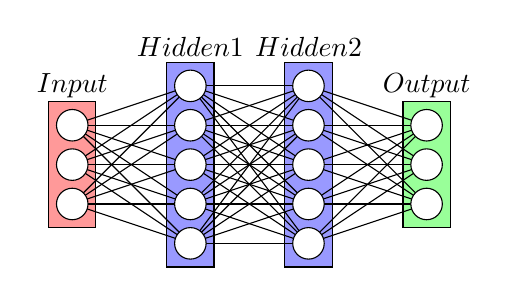
\begin{tikzpicture}[scale=1, transform shape]
  \node (i0) at (0.0,-0.5) {};
  \node (i1) at (0.0,0.0) {};
  \node (i2) at (0.0,0.5) {};

  \node (h00) at (1.5,-1.0) {};
  \node (h01) at (1.5,-0.5) {};
  \node (h02) at (1.5,0.0) {};
  \node (h03) at (1.5,0.5) {};
  \node (h04) at (1.5,1.0) {};

  \node (h10) at (3.0,-1.0) {};
  \node (h11) at (3.0,-0.5) {};
  \node (h12) at (3.0,0.0) {};
  \node (h13) at (3.0,0.5) {};
  \node (h14) at (3.0,1.0) {};

  \node (o0) at (4.5, -0.5) {};
  \node (o1) at (4.5, 0.0) {};
  \node (o2) at (4.5, 0.5) {};

  \node (i) at (0.0,1.0) {$Input$};
  \node (h0) at (1.5,1.5) {$Hidden 1$};
  \node (h0) at (3.0,1.5) {$Hidden 2$};
  \node (i) at (4.5,1.0) {$Output$};

  \filldraw[fill=red!40!white] (-0.3,-0.8) rectangle (0.3, 0.8);

  \filldraw[fill=blue!40!white] (1.2,-1.3) rectangle (1.8, 1.3);
  \filldraw[fill=blue!40!white] (2.7,-1.3) rectangle (3.3, 1.3);

  \filldraw[fill=green!40!white] (4.2,-0.8) rectangle (4.8, 0.8);

  \draw (i0) -- (h00);
  \draw (i0) -- (h01);
  \draw (i0) -- (h02);
  \draw (i0) -- (h03);
  \draw (i0) -- (h04);

  \draw (i1) -- (h00);
  \draw (i1) -- (h01);
  \draw (i1) -- (h02);
  \draw (i1) -- (h03);
  \draw (i1) -- (h04);

  \draw (i2) -- (h00);
  \draw (i2) -- (h01);
  \draw (i2) -- (h02);
  \draw (i2) -- (h03);
  \draw (i2) -- (h04);

  \draw (h00) -- (h10);
  \draw (h00) -- (h11);
  \draw (h00) -- (h12);
  \draw (h00) -- (h13);
  \draw (h00) -- (h14);

  \draw (h01) -- (h10);
  \draw (h01) -- (h11);
  \draw (h01) -- (h12);
  \draw (h01) -- (h13);
  \draw (h01) -- (h14);

  \draw (h02) -- (h10);
  \draw (h02) -- (h11);
  \draw (h02) -- (h12);
  \draw (h02) -- (h13);
  \draw (h02) -- (h14);

  \draw (h03) -- (h10);
  \draw (h03) -- (h11);
  \draw (h03) -- (h12);
  \draw (h03) -- (h13);
  \draw (h03) -- (h14);

  \draw (h04) -- (h10);
  \draw (h04) -- (h11);
  \draw (h04) -- (h12);
  \draw (h04) -- (h13);
  \draw (h04) -- (h14);

  \draw (h10) -- (o0);
  \draw (h10) -- (o1);
  \draw (h10) -- (o2);

  \draw (h11) -- (o0);
  \draw (h11) -- (o1);
  \draw (h11) -- (o2);

  \draw (h12) -- (o0);
  \draw (h12) -- (o1);
  \draw (h12) -- (o2);

  \draw (h13) -- (o0);
  \draw (h13) -- (o1);
  \draw (h13) -- (o2);

  \draw (h14) -- (o0);
  \draw (h14) -- (o1);
  \draw (h14) -- (o2);

  \filldraw[fill=white] (i0) circle (0.2);
  \filldraw[fill=white] (i1) circle (0.2);
  \filldraw[fill=white] (i2) circle (0.2);

  \filldraw[fill=white] (h00) circle (0.2);
  \filldraw[fill=white] (h01) circle (0.2);
  \filldraw[fill=white] (h02) circle (0.2);
  \filldraw[fill=white] (h03) circle (0.2);
  \filldraw[fill=white] (h04) circle (0.2);

  \filldraw[fill=white] (h10) circle (0.2);
  \filldraw[fill=white] (h11) circle (0.2);
  \filldraw[fill=white] (h12) circle (0.2);
  \filldraw[fill=white] (h13) circle (0.2);
  \filldraw[fill=white] (h14) circle (0.2);

  \filldraw[fill=white] (o0) circle (0.2);
  \filldraw[fill=white] (o1) circle (0.2);
  \filldraw[fill=white] (o2) circle (0.2);
\end{tikzpicture}

  \end{center}
  \captionof{figure}{Example structure of a two layer neural network, with the
  four layers highlighted in different colors.}
  \label{fig:nn_two_layer}
  \end{Figure}

  In figure \ref{fig:nn_two_layer} an example of how each layer of neurons
  interact with one another can be seen. Note how each neuron of the previous
  layer is now an input for every neuron of the current layer. We call this
  type of network a "two layer" network even though it clearly has four layers.
  This is because the input and output layers must always be present, and so it
  is not important if we count them or not, thus the important number is the
  number of hidden layers in the network.

  There are many different types of layers that can be utilized together in a
  neural network. This introduction will provide a brief introduction to many
  of the commonly implemented types of layers, but will only go into specific
  detail and implementation of a select few of the layer types.

  \begin{description}
    \item[Input] The input layer reads the data from the user and then passes
      that on to the next layer in the network. This layer does no computation
      on its own, it is only used as a house keeping tool to keep everything
      concise and organized.
    \item[Output] The output layer takes the values that are determined by the
      previous layers of the network, and provides them to the user.
    \item[Dense] A dense or fully connected layer is what we will mainly be
      focusing on. A dense layer means that each neuron in the layer is
      connected to every neuron in the previous layer and every neuron in the
      next layer. For this introduction to neural networks, this is where the
      core of the computation is preformed. The computation of this layer is
      \[
        f((W\cdot V) + b)
      \]
      where $f$ is the activation function for the layer, $W$ is the matrix of
      weights for the dense layer, sometimes called the kernel, $V$ is the
      vector of input values passed to the layer by the previous layer, and $b$
      is the vector of bias values that are applied to the product of the
      weights and input.
    \item[Activation] This layer is a tool that can be used to apply special
      activation functions, beyond what is normally applied by the dense layer.
      This means that this layer simply computes
      \[
        f(V)
      \]
      where $f$ is some activation function, and $V$ is the vector of input
      values.
    \item[Dropout] Dropout is a more advanced tool that is used to prevent
      over fitting during the training stages. It randomly sets some
      percentages of the input values to $0$ before passing them on.
    \item[Reshape] This is a utility layer that is used for when the input data
      may not be a strict vector of values. For example if the input is an
      image with a red, green, and blue channel, then the input would be a
      three dimensional matrix of values. The reshape layer allows the user to
      reshape the data into whatever format is necessary for the later layers
      of the network. So to pass an image into a dense layer, one would reshape
      the three dimensional matrix into a one dimensional matrix or vector.
    \item[Convolutional] The convolutional layer is a key part of most image
      recognition neural networks. The convolutional layer applies a matrix of
      weights over a small region of the input values, then by some means of
      moving the region that it will apply the matrix, the process is repeated
      to cover the entirety of the input values. There are many nuances of
      this type of layer that must be considered for proper implementation.
    \item[Pooling] The pooling layer is intended to quickly reduce the scale of
      the data that is begin passed through the network, by some method. The
      pooling layer takes the input values and outputs a significantly reduced
      size of output values. There are two ways that this commonly done. Either
      by taking the $max$ of several values in the input layer, or by taking
      the $avg$ of those values. Either way, this layer takes many values and
      condenses them down into a single value, either though maximum, or
      averaging.
  \end{description}

  \section{Deep Feed Forward Network}%
  \label{sec:deep_feed_forward_network}

  The Deep Feed Forward (DFF) network, is one of the simplest networks, and so
  is a great choice for an introduction to how to construct a neural network. A
  typical representation of a DFF is depicted in figure \ref{fig:dff}. The
  network in the depiction has one input layer, two dense layers, and one
  output layer. We will used this specific network for most of the explanation,
  but it can easily be generalized to larger networks.

  \begin{Figure}
  \begin{center}
    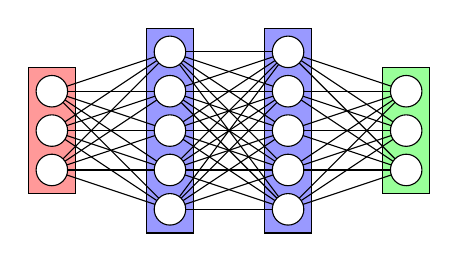
\begin{tikzpicture}[scale=1, transform shape]
  \node (i0) at (0.0,-0.5) {};
  \node (i1) at (0.0,0.0) {};
  \node (i2) at (0.0,0.5) {};

  \node (h00) at (1.5,-1.0) {};
  \node (h01) at (1.5,-0.5) {};
  \node (h02) at (1.5,0.0) {};
  \node (h03) at (1.5,0.5) {};
  \node (h04) at (1.5,1.0) {};

  \node (h10) at (3.0,-1.0) {};
  \node (h11) at (3.0,-0.5) {};
  \node (h12) at (3.0,0.0) {};
  \node (h13) at (3.0,0.5) {};
  \node (h14) at (3.0,1.0) {};

  \node (o0) at (4.5, -0.5) {};
  \node (o1) at (4.5, 0.0) {};
  \node (o2) at (4.5, 0.5) {};

  \filldraw[fill=red!40!white] (-0.3,-0.8) rectangle (0.3, 0.8);

  \filldraw[fill=blue!40!white] (1.2,-1.3) rectangle (1.8, 1.3);
  \filldraw[fill=blue!40!white] (2.7,-1.3) rectangle (3.3, 1.3);

  \filldraw[fill=green!40!white] (4.2,-0.8) rectangle (4.8, 0.8);

  \draw (i0) -- (h00);
  \draw (i0) -- (h01);
  \draw (i0) -- (h02);
  \draw (i0) -- (h03);
  \draw (i0) -- (h04);

  \draw (i1) -- (h00);
  \draw (i1) -- (h01);
  \draw (i1) -- (h02);
  \draw (i1) -- (h03);
  \draw (i1) -- (h04);

  \draw (i2) -- (h00);
  \draw (i2) -- (h01);
  \draw (i2) -- (h02);
  \draw (i2) -- (h03);
  \draw (i2) -- (h04);

  \draw (h00) -- (h10);
  \draw (h00) -- (h11);
  \draw (h00) -- (h12);
  \draw (h00) -- (h13);
  \draw (h00) -- (h14);

  \draw (h01) -- (h10);
  \draw (h01) -- (h11);
  \draw (h01) -- (h12);
  \draw (h01) -- (h13);
  \draw (h01) -- (h14);

  \draw (h02) -- (h10);
  \draw (h02) -- (h11);
  \draw (h02) -- (h12);
  \draw (h02) -- (h13);
  \draw (h02) -- (h14);

  \draw (h03) -- (h10);
  \draw (h03) -- (h11);
  \draw (h03) -- (h12);
  \draw (h03) -- (h13);
  \draw (h03) -- (h14);

  \draw (h04) -- (h10);
  \draw (h04) -- (h11);
  \draw (h04) -- (h12);
  \draw (h04) -- (h13);
  \draw (h04) -- (h14);

  \draw (h10) -- (o0);
  \draw (h10) -- (o1);
  \draw (h10) -- (o2);

  \draw (h11) -- (o0);
  \draw (h11) -- (o1);
  \draw (h11) -- (o2);

  \draw (h12) -- (o0);
  \draw (h12) -- (o1);
  \draw (h12) -- (o2);

  \draw (h13) -- (o0);
  \draw (h13) -- (o1);
  \draw (h13) -- (o2);

  \draw (h14) -- (o0);
  \draw (h14) -- (o1);
  \draw (h14) -- (o2);

  \filldraw[fill=white] (i0) circle (0.2);
  \filldraw[fill=white] (i1) circle (0.2);
  \filldraw[fill=white] (i2) circle (0.2);

  \filldraw[fill=white] (h00) circle (0.2);
  \filldraw[fill=white] (h01) circle (0.2);
  \filldraw[fill=white] (h02) circle (0.2);
  \filldraw[fill=white] (h03) circle (0.2);
  \filldraw[fill=white] (h04) circle (0.2);

  \filldraw[fill=white] (h10) circle (0.2);
  \filldraw[fill=white] (h11) circle (0.2);
  \filldraw[fill=white] (h12) circle (0.2);
  \filldraw[fill=white] (h13) circle (0.2);
  \filldraw[fill=white] (h14) circle (0.2);

  \filldraw[fill=white] (o0) circle (0.2);
  \filldraw[fill=white] (o1) circle (0.2);
  \filldraw[fill=white] (o2) circle (0.2);
\end{tikzpicture}

  \end{center}
  \captionof{figure}{Deep Feed Forward Neural Network.}
  \label{fig:dff}
  \end{Figure}

  One key aspect of a DFF network, is that it only consists of a single input
  and output layer, with some number of dense layers in between the two.

  \subsection{Forward Propagation}%
  \label{sub:forward_propagation}

  Forward propagation is the process of taking values for the input layer, and
  using the matrix to determine the values of the output layer. This process
  does not train the network in any way, it is just using the network to
  determine outputs for a given input. When a network is actually placed into
  production, this is the process that is being used.

  As demonstrated in section \ref{sub:neuron}, each neuron computes
  \begin{align*}
    f(w_1x_1+w_2x_2+\ldots+w_nx_n+b).
  \end{align*}
  And we note that here $f$ is any activation function.

  Then since each layer has many neurons, it is helpful to consider the layer
  as a whole instead of a single neuron at a time. For this example we will
  consider the first dense layer in the network. This means that each neuron is
  taking in $3$ inputs from the three input neurons. We denote the neuron in
  the layer using $i$, using this notation, each neuron computes
  \begin{align*}
    f(w_{i1}x_1+w_{i2}x_2+w_{i3}x_3+b_i)\quad i=1,\ldots,5.
  \end{align*}
  Since this operation is begin done for every $i$, it can be easily seen that
  it matches a matrix expression of
  \begin{align*}
    f\left(\begin{pmatrix}
        w_{11} & w_{12} & w_{13}\\
        w_{21} & w_{22} & w_{23}\\
        w_{31} & w_{32} & w_{33}\\
        w_{41} & w_{42} & w_{43}\\
        w_{51} & w_{52} & w_{53}\\
      \end{pmatrix}
      \begin{pmatrix}
        x_1 \\
        x_2 \\
        x_3
      \end{pmatrix}+
      \begin{pmatrix}
        b_1\\
        b_2\\
        b_3\\
        b_4\\
        b_5
      \end{pmatrix}
    \right).
  \end{align*}
  Where $f$ of a vector is the same as taking $f$ of each element individually.
  This notation is usually written in the form
  \begin{align}\label{eq:dense_f}
    f\left(W\cdot X+B\right).
  \end{align}
  Since this is the function for the first dense layer we will denote that by
  the use of an index. Thus the expression for the computation done by the
  first layer is
  \begin{align*}
    f^{(1)}\left(W^{(1)}\cdot X+B^{(1)}\right).
  \end{align*}
  This is the final output of the values of the neurons from the first layer.

  Since the second dense layer uses the first dense layer as the inputs, then
  the equation \ref{eq:dense_f} for the first layer becomes the new $X$ vector.
  For a small network such as this one, it is possible to write the complete
  expression for the second dense layer. We find this to be
  \begin{align*}
    f^{(2)}\left(W^{(2)}\cdot\left[f^{(1)}\left(W^{(1)}\cdot
    X+B^{(1)}\right)\right]+B^{(2)}\right).
  \end{align*}
  This expression can be chained for as many hidden layers as the deep feed
  forward network has. That is until one reaches the output layer. In most
  cases the output layer also acts as a dense layer in order to reshape the
  data into the desired output shape.

  For our example problem, we will treat the output layer exactly as another
  dense layer. Thus the final expression becomes
  \begin{align*}
    \resizebox{\columnwidth}{!}{$
    f^{(o)}\left(W^{(o)}\cdot f^{(2)}\left(W^{(2)}\cdot f^{(1)}\left(
  W^{(1)}\cdot X+B^{(1)}\right)+B^{(2)}\right)+B^{(o)}\right)$}.
  \end{align*}

  Looking into the details of the $W$ and the $B$ matrices, it can clearly be
  seen that the dimensions of $W^{(1)}$ is $5\times 3$ matrix, $B^{(1)}$ is
  $5\times 1$, $W^{(2)}$ is $5\times 5$, $B^{(2)}$ is $5\times 1$, $W^{(o)}$ is
  $3\times 5$ and $B^{(o)}$ is $3\times 1$. These dimensions were just
  determined by what they must be in order for the matrix multiplication to
  even make any sense.

  An alternative way to structure a dense layer, is to add a value of $1$ to
  the input vector, and to place the bias vector into the weights matrix. This
  can be written as
  \begin{align*}
    f\left(\begin{pmatrix}
        w_{11} & w_{12} & w_{13} & b_1\\
        w_{21} & w_{22} & w_{23} & b_2\\
        w_{31} & w_{32} & w_{33} & b_3\\
        w_{41} & w_{42} & w_{43} & b_3\\
        w_{51} & w_{52} & w_{53} & b_5\\
      \end{pmatrix}
      \begin{pmatrix}
        x_1 \\
        x_2 \\
        x_3 \\
        1
      \end{pmatrix}
    \right).
  \end{align*}
  This provides the computational benefit of only needing to do a single
  operation of matrix multiplication, versus a matrix multiplication and vector
  addition operation. Because of this equivalent representation of the formula,
  the bias vector is often implicitly included into the weights matrix. Thus
  the formula would be written as
  \begin{align}\label{eq:dense_f2}
    f(W\cdot X),
  \end{align}
  and the bias terms should be inferred to be present in the weights matrix.

  \subsection{Initialization}%
  \label{sub:initialization}

  As it should be understood now, each dense layer must have a matrix of
  $N\times (M+1)$ where $N$ is the number of neurons in the layer, and $M$ is
  the number of neurons in the previous layer. Before it is possible to train a
  network, we need an initial condition. This means that we must determine some
  method for constructing the initial values of the weight matrices.

  For this process, we consider three methods
  \begin{description}
    \item[Zeros] It is reasonable thinking that half of the weights of a
      network will be positive, and about half will be negative. Thus it would
      make sense to initialize the weights as zero, which would be about the
      average weight. The pitfall of this method, is that each neuron would be
      trained exactly the same. This would means that each neuron and each
      weight for each neuron would be altered in the exact same way, and
      wouldn't allow for any variations between one another.
    \item[Small Random] A method that can be employed to avoid the issues that
      arise with zero initialized weights, is to initialize using small random
      values. This way the weights are still near zero, but each weight will be
      distinct, and learn different things, leading to a more powerful network.
  \end{description}

\end{multicols}

\end{document}
